\documentclass[border=5pt]{standalone}
\usepackage{tikz}
\usepackage{times}
\usetikzlibrary{positioning,shapes.geometric,arrows.meta,backgrounds,fit,calc}

\begin{document}

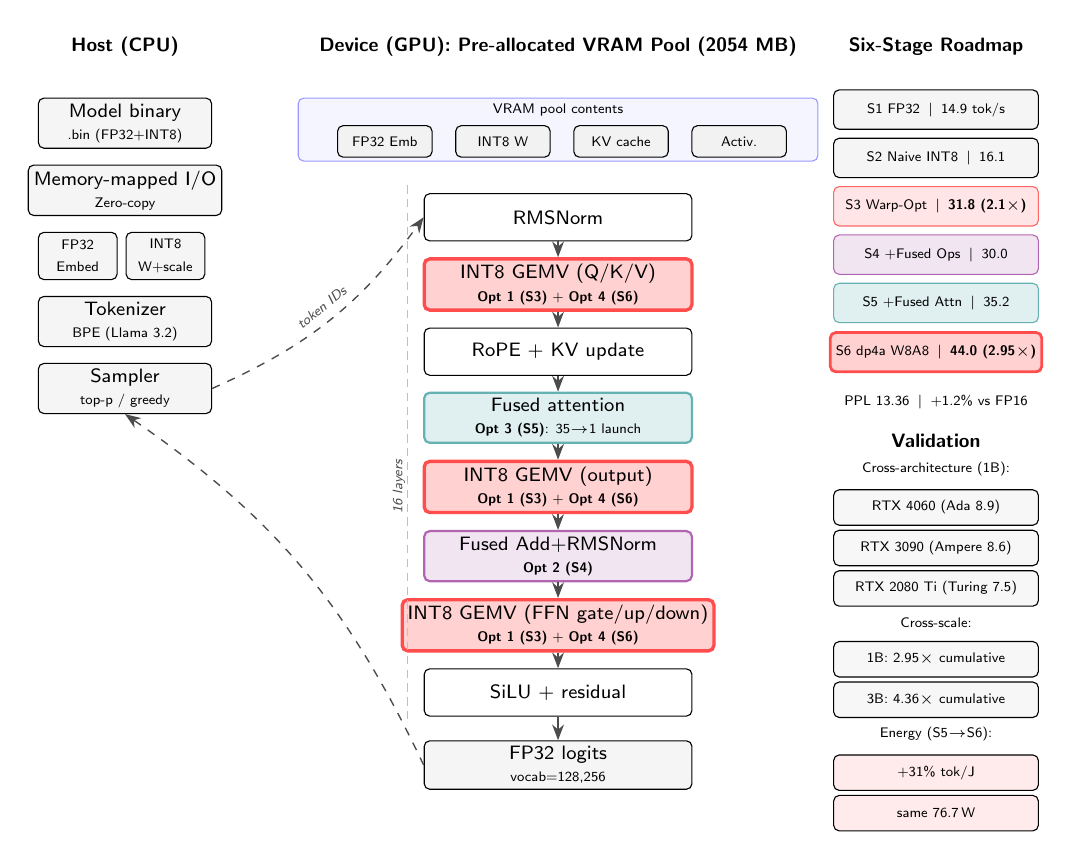
\begin{tikzpicture}[
    font=\sffamily\footnotesize,
    >={Stealth[length=2mm,width=1.5mm]},
    box/.style={
        draw=black,
        line width=0.4pt,
        rounded corners=2pt,
        minimum height=6mm,
        minimum width=22mm,
        align=center,
        inner sep=2pt,
        font=\sffamily\scriptsize
    },
    hostbox/.style={box, fill=gray!8},
    pipebox/.style={box, fill=white, minimum width=34mm},
    optred/.style={box, fill=red!10, draw=red!60, line width=0.8pt, minimum width=34mm},
    optredbold/.style={box, fill=red!18, draw=red!70, line width=1.2pt, minimum width=34mm},
    optpurple/.style={box, fill=violet!10, draw=violet!60, line width=0.8pt, minimum width=34mm},
    optteal/.style={box, fill=teal!12, draw=teal!60, line width=0.8pt, minimum width=34mm},
    stagebox/.style={box, minimum width=26mm, minimum height=5mm, font=\sffamily\tiny},
    validbox/.style={box, minimum width=26mm, minimum height=4.5mm, font=\sffamily\tiny, fill=gray!6},
    arr/.style={->, line width=0.5pt, draw=black!70},
    label/.style={font=\sffamily\tiny\itshape, text=black!70},
    title/.style={font=\sffamily\scriptsize\bfseries}
]

% ==================== Section labels ====================
\node[title] (lab_host) at (0, 0) {Host (CPU)};
\node[title] (lab_dev) at (5.5, 0) {Device (GPU): Pre-allocated VRAM Pool (2054 MB)};
\node[title] (lab_road) at (10.3, 0) {Six-Stage Roadmap};

% ==================== HOST COLUMN (left) ====================
\node[hostbox, below=4mm of lab_host] (bin) {Model binary\\ \tiny .bin (FP32+INT8)};
\node[hostbox, below=2mm of bin] (mmap) {Memory-mapped I/O\\ \tiny Zero-copy};

% FP32 / INT8 side by side
\node[hostbox, below=2mm of mmap, xshift=-6mm, minimum width=10mm] (fp) {\tiny FP32\\ \tiny Embed};
\node[hostbox, right=1mm of fp, minimum width=10mm] (i8) {\tiny INT8\\ \tiny W+scale};

\node[hostbox, below=2mm of fp, xshift=6mm] (tok) {Tokenizer\\ \tiny BPE (Llama 3.2)};
\node[hostbox, below=2mm of tok] (sampler) {Sampler\\ \tiny top-p / greedy};

% ==================== DEVICE COLUMN (center) ====================
% VRAM pool summary row
\node[box, fill=blue!4, draw=blue!40, minimum width=66mm, minimum height=8mm, below=4mm of lab_dev] (pool) {};
\node[font=\sffamily\tiny] at ([yshift=2.5mm] pool.center) {VRAM pool contents};
\node[box, fill=gray!10, minimum width=12mm, minimum height=4mm, font=\sffamily\tiny]
    at ([yshift=-1.5mm, xshift=-22mm] pool.center) {FP32 Emb};
\node[box, fill=gray!10, minimum width=12mm, minimum height=4mm, font=\sffamily\tiny]
    at ([yshift=-1.5mm, xshift=-7mm] pool.center) {INT8 W};
\node[box, fill=gray!10, minimum width=12mm, minimum height=4mm, font=\sffamily\tiny]
    at ([yshift=-1.5mm, xshift=8mm] pool.center) {KV cache};
\node[box, fill=gray!10, minimum width=12mm, minimum height=4mm, font=\sffamily\tiny]
    at ([yshift=-1.5mm, xshift=23mm] pool.center) {Activ.};

% Transformer pipeline
\node[pipebox, below=4mm of pool] (rmsnorm) {RMSNorm};
\node[optredbold, below=2mm of rmsnorm] (gemv1) {INT8 GEMV (Q/K/V)\\ \tiny \textbf{Opt 1 (S3)} + \textbf{Opt 4 (S6)}};
\node[pipebox, below=2mm of gemv1] (rope) {RoPE + KV update};
\node[optteal, below=2mm of rope] (attn) {Fused attention\\ \tiny \textbf{Opt 3 (S5)}: 35$\to$1 launch};
\node[optredbold, below=2mm of attn] (gemv2) {INT8 GEMV (output)\\ \tiny \textbf{Opt 1 (S3)} + \textbf{Opt 4 (S6)}};
\node[optpurple, below=2mm of gemv2] (rms2) {Fused Add+RMSNorm\\ \tiny \textbf{Opt 2 (S4)}};
\node[optredbold, below=2mm of rms2] (gemv3) {INT8 GEMV (FFN gate/up/down)\\ \tiny \textbf{Opt 1 (S3)} + \textbf{Opt 4 (S6)}};
\node[pipebox, below=2mm of gemv3] (silu) {SiLU + residual};

% Layer x 16 indicator
\draw[densely dashed, gray!50, line width=0.4pt]
    ([xshift=-2mm, yshift=1mm] rmsnorm.north west) --
    ([xshift=-2mm, yshift=-1mm] silu.south west);
\node[label, rotate=90] at ([xshift=-3mm] $(gemv2.west)$) {16 layers};

% Final output
\node[pipebox, below=3mm of silu, fill=gray!8] (logits) {FP32 logits\\ \tiny vocab=128{,}256};

% Arrows in pipeline
\foreach \a/\b in {rmsnorm/gemv1, gemv1/rope, rope/attn, attn/gemv2, gemv2/rms2,
                    rms2/gemv3, gemv3/silu, silu/logits}{
    \draw[arr] (\a) -- (\b);
}

% ==================== Host <-> Device arrows ====================
\draw[arr, dashed] (sampler.east) to[bend right=15]
    node[label, above, sloped, midway] {token IDs} (rmsnorm.west);
\draw[arr, dashed] (logits.west) to[bend right=15] (sampler.south);

% ==================== Right side: roadmap ====================
\begin{scope}[xshift=10.3cm, yshift=-0.8cm]
    \node[stagebox, fill=gray!8] (s1) at (0, 0) {S1 FP32 \,\textbar\, 14.9 tok/s};
    \node[stagebox, fill=gray!8, below=1mm of s1] (s2) {S2 Naive INT8 \,\textbar\, 16.1};
    \node[stagebox, fill=red!10, draw=red!60, below=1mm of s2] (s3) {S3 Warp-Opt \,\textbar\, \textbf{31.8 (2.1$\times$)}};
    \node[stagebox, fill=violet!10, draw=violet!60, below=1mm of s3] (s4) {S4 +Fused Ops \,\textbar\, 30.0};
    \node[stagebox, fill=teal!12, draw=teal!60, below=1mm of s4] (s5) {S5 +Fused Attn \,\textbar\, 35.2};
    \node[stagebox, fill=red!18, draw=red!70, line width=1pt, below=1mm of s5] (s6) {S6 dp4a W8A8 \,\textbar\, \textbf{44.0 (2.95$\times$)}};
    \node[font=\sffamily\tiny, below=1.5mm of s6] (pplnote) {PPL 13.36 \,\textbar\, +1.2\% vs FP16};
\end{scope}

% ==================== Right side: validation panel ====================
\begin{scope}[xshift=10.3cm, yshift=-5cm]
    \node[title, font=\sffamily\scriptsize\bfseries] (valtitle) {Validation};

    \node[font=\sffamily\tiny, below=1.5mm of valtitle, anchor=center] (crossarch) {Cross-architecture (1B):};
    \node[validbox, below=0.5mm of crossarch] (g4060) {RTX 4060 (Ada 8.9)};
    \node[validbox, below=0.5mm of g4060] (g3090) {RTX 3090 (Ampere 8.6)};
    \node[validbox, below=0.5mm of g3090] (g2080) {RTX 2080 Ti (Turing 7.5)};

    \node[font=\sffamily\tiny, below=2mm of g2080, anchor=center] (crossscale) {Cross-scale:};
    \node[validbox, below=0.5mm of crossscale] (m1b) {1B: 2.95$\times$ cumulative};
    \node[validbox, below=0.5mm of m1b] (m3b) {3B: 4.36$\times$ cumulative};

    \node[font=\sffamily\tiny, below=2mm of m3b, anchor=center] (energy) {Energy (S5$\to$S6):};
    \node[validbox, below=0.5mm of energy, fill=red!8] (e1) {+31\% tok/J};
    \node[validbox, below=0.5mm of e1, fill=red!8] (e2) {same 76.7\,W};
\end{scope}

% Legend removed — covered by figure caption

\end{tikzpicture}
\end{document}
